%% OJEPN article template for LaTeX
%% Licence: Creative Commons Attribution Share-Alike 4.0
%% Author:  Andy J. Wills
%% Adapted from a Creative Commons template by Jonathan Baron

\documentclass[twocolumn]{article}
\usepackage[utf8]{inputenc}
\usepackage[T1]{fontenc}
\usepackage[english]{babel}
\usepackage{ifpdf,amsmath,amsthm,amssymb,amsfonts,newtxtext,newtxmath} 
\usepackage{array,graphicx,dcolumn,multirow,hevea,abstract,hanging}
\usepackage[labelfont=sc,textfont=sf]{caption}
\usepackage[hyperfootnotes=false,breaklinks=true,hidelinks]{hyperref} % was dvipdfmx
\urlstyle{rm}
\usepackage[hyphenbreaks]{breakurl}
%\usepackage{natbib} % must come afer hyperfootnotes
%\setlength{\bibsep}{0pt}
\usepackage{booktabs} % \toprule \midrule \bottomrule \cmidrule(lr){a-b}
% define centered and ragged columns:
\newcolumntype{L}[1]{>{\raggedright\arraybackslash }p{#1}} % can use m{}
\newcolumntype{C}[1]{>{\centering\arraybackslash }p{#1}}
\newcolumntype{R}[1]{>{\raggedleft\arraybackslash }p{#1}}
\newcolumntype{d}[1]{D{.}{.}{#1}} % d{3.2} for 3 places on l, 2 on r
\newcommand{\mc}{\multicolumn}
\topmargin=-.3in \oddsidemargin=-.1in \evensidemargin=-.1in \textheight=9in \textwidth=6.8in
\setlength\tabcolsep{1mm}
\setlength\columnsep{5mm}
\setlength\abovecaptionskip{1ex}
\setlength\belowcaptionskip{.5ex}
\setlength\belowbottomsep{.3ex}
\setlength\lightrulewidth{.04em}
\renewcommand\arraystretch{1.2}
\renewcommand{\topfraction}{1}
\renewcommand{\textfraction}{0}
\renewcommand{\floatpagefraction}{.9}
% \renewcommand{\baselinestretch}{1.00} \large\normalsize % for fixing spaces
\widowpenalty=1000
\clubpenalty=1000
\setlength{\parskip}{0ex}
\let\tempone\itemize
\let\temptwo\enditemize


\let\tempthree\enumerate
\let\tempfour\endenumerate
\renewenvironment{itemize}{\tempone\setlength{\itemsep}{0pt}}{\temptwo}
\renewenvironment{enumerate}{\tempthree\setlength{\itemsep}{0pt}}{\tempfour}
\usepackage{setspace}

\usepackage[natbibapa]{apacite}
\setlength{\bibhang}{0.5cm}

\usepackage{xspace}
\newcommand*{\eg}{e.g.\@\xspace}
\newcommand*{\ie}{i.e.\@\xspace}

\usepackage{xcolor}

%%%%%%%%%%%%%%%%%%%%%%%%%%%%%%%%%%%%%%%%%%%%%%%%%%%%%%%%%%%%%%%%%%%%%
\setcounter{page}{3} % start with first page

\title{Absence of cross-modality analogical transfer in perceptual categorization}

\author{
C. E. R. Edmunds\thanks{School of Biological and Chemical Sciences, Queen Mary, University of London, U.K. Email: ceredmunds@gmail.com}
\and
Angus B. Inkster\thanks{School of Psychology, University of Plymouth, U.K.}
\and 
Peter M. Jones\footnotemark[2]
\and
Fraser Milton\thanks{School of Psychology, University of Exeter, U.K.} % indicates same as 2nd thanks
\and
Andy J. Wills\footnotemark[2]
}

\date{} % leave empty
\begin{document} % goes here

% fill in short title
\newcommand{\jhead}{Open Journal of Experimental Psychology and Neuroscience, 2020}
\newcommand{\jdate}{Vol.~1}
\pagestyle{myheadings} \markright{\protect\small \jhead, \jdate \hfill ABSENCE OF TRANSFER \qquad}
\begin{htmlonly}
%\href{\jref}{\jhead}, \jdate, pp.\
\end{htmlonly}
%\begin{latexonly}
\twocolumn[
\vspace{-.3in}
{\small \jhead, \jdate, pp.\ 3--13. \hfill \url{https://doi.org/10.46221/ojepn.2020.8639}}
%\end{latexonly}

\maketitle
%\doublespacing

%\begin{latexonly}
\vspace{-3mm}
\begin{onecolabstract}
%\end{latexonly}

Analogical transfer has been previously reported to occur between rule-based, but not information-integration, perceptual category structures \citep{Casale:2012jf}. The current study investigated whether a similar pattern of results would be observed in cross-modality transfer. Participants were trained on either a rule-based structure, or an information-integration structure, using visual stimuli. They were then tested on auditory stimuli that had the same underlying abstract category structure. Transfer performance was assessed relative to a control group who did not receive training on the visual stimuli. No cross-modality transfer was found, irrespective of the category structure employed.

\smallskip
\noindent
Keywords: analogical reasoning, generalisation, strategies, learning, multiple systems
%\begin{latexonly}
\end{onecolabstract}\bigskip
]
%\end{latexonly}

{\renewcommand{\thefootnote}{}
\footnotetext{ % note blank lines above and below acknowledgment

  Thanks to Hayley Robinson and Sophia Pearn for running one of the pilot experiments and to Madeline Bartlett for coding of the verbal reports.

Copyright: \copyright\ 2020.
The authors license this article under the terms of the
\href{http://creativecommons.org/licenses/by/3.0/}{Creative Commons
  Attribution Share-Alike 4.0 License.}
}}

\saythanks

\setlength{\baselineskip}{12pt plus.2pt}

\section{Introduction}

%\doublespacing

Analogical transfer is the ability to transfer knowledge of structural features of a problem from one domain to another \citep{Gentner:2018wo}. The canonical example \citep{Gick1980} asked: ``how do you destroy a tumor using intense radiation without damaging the surrounding tissue?'' \citep{Duncker1945}. People found this easier to solve if they had previously experienced an analogous problem in a military context (``how can you storm a castle with a large army when the surrounding bridges are weak?''). Obviously, the worth of transferring knowledge extends far beyond satisfying the whims of experimental psychologists. For instance, it is central to scientific work, from hypothesis generation to data interpretation \citep{Dunbar:1997wd}. Further, without analogical transfer much of the effectiveness of education is lost \citep{Ford:2018gm}. After all, who would trust a nurse \citep{Johnston:2017ct} or engineer \citep{Chase:2019fb} who is unable to generalise their training? 

In the transfer literature, one rarely-explored task is perceptual categorization, where people learn to label groups of perceptually similar stimuli \citep{Kurtz:2015ew}. For instance, a doctor might categorize scans as showing evidence of cancer or remission \citep{Hornsby:2014jy}. Analogical transfer research on perceptual categorization has solely examined unidimensional and information-integration tasks \citep[see Figure~\ref{figure:categoryStructures};][]{Ashby1988}.\footnote{There has also been work examining the transfer of relational categories which is outside the definition of perceptual categorization used here.} For ease of exposition, assume we are categorizing Gabor patches varying in the number and orientation of bars. In unidimensional (UD) tasks (see Figure~\ref{figure:categoryStructures}A), participants sort stimuli using a single dimension: ``Patches with bars orientated less than 45 degrees are in Category A; otherwise they are in Category B.'' In contrast, in information-integration (II) tasks (see Figure~\ref{figure:categoryStructures}B) participants combine features from two incommensurable dimensions.\footnote{II structures are difficult to describe. However, for those interested, a possible description of an II category in Gabor patch stimuli is ``If there are more bars than the bars are upright then the stimulus is in Category A, otherwise it is in B.'' This description sounds nonsensical and so is unlikely to be identified by participants.} These two tasks are rotations of each other in stimulus space and so are argued to be well-matched on between-category distance, within-category similarity and difficulty (\eg \citeauthor{Smith:2014ec}, \citeyear{Smith:2014ec}; \citeauthor{Ashby2018}, \citeyear{Ashby2018}; although see \citeauthor{Newell2011a}, \citeyear{Newell2011a}). Indeed, a large literature has been built on the assumption that the principal difference between these two structures is that they differ in how easy it is to describe the decision-boundary between the categories \citep{Ashby2005, Ashby2011, Ashby2016a}. 

\begin{figure*}[t!]
	\centering
	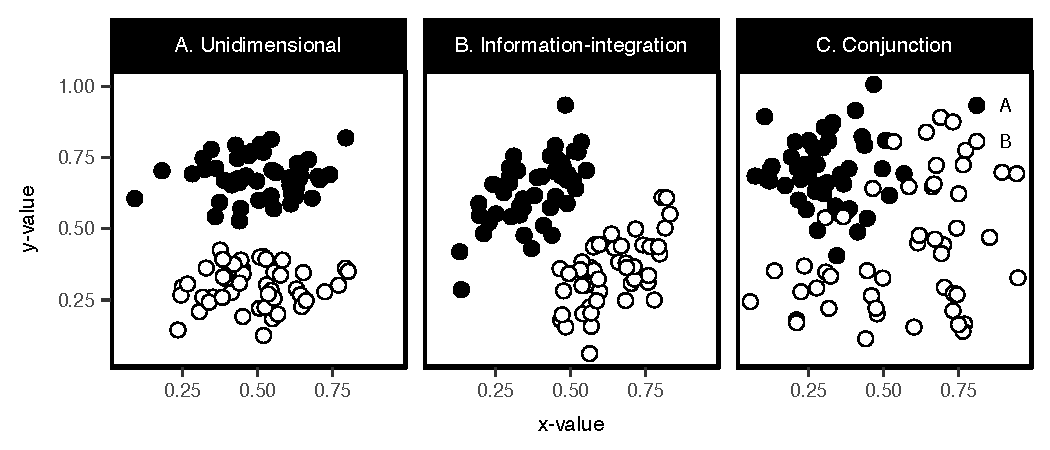
\includegraphics[width=\textwidth]{images/CategoryStructures}
	\caption{Examples of A. Unidimensional, B. Information-integration and C. conjunction category structures. Each circle represents a stimulus. Filled
circles indicate stimuli belonging to Category~A, and empty circles those
belonging to Category~B.}
	\label{figure:categoryStructures}
\end{figure*}

Despite their many similarities, these categorization tasks do not appear to be equally amenable to analogical transfer. In this context, analogical transfer would be shown ``if a participant is able to apply a classification strategy learned with one set of stimuli to a set of novel, perceptually distinct stimuli'' \citep[p. 434]{Casale:2012jf}. In \citeauthor{Casale:2012jf}'s \citeyearpar{Casale:2012jf} experiments, participants learned to categorize Gabor patch stimuli according to a UD or II structure. To test the extent of analogical transfer, participants then completed similar categorization tasks with stimuli perceptually distinct from the training set. These novel test stimuli were chosen such that the between-category decision boundary was the same for both sets of stimuli. Across three experiments \citeauthor{Casale:2012jf} found that participants who learned a UD structure could transfer that knowledge to another stimulus space region. However, those who learned an II structure could not. In a similar study that used rectangles of visual static (random green dots) that varied in dot density and rectangle size, \cite{Zakrzewski:2018gu} found the same pattern \citep[see also][]{Soto:2018up}.

In summary, previous studies indicate that analogical transfer is possible for UD tasks but not for II tasks. However, these studies limit the inferences we can make about analogical transfer as they are all examples of so-called ``near transfer,'' where both tasks are presented in a similar context, using similar stimuli \citep{Barnett:2002io}. Of more interest is ``far transfer,'' such as the radiation problem mentioned above, where the surface task features differ between training and test. After all, the more situations to which we can transfer knowledge, the more use it is. Therefore, in the current work we investigate far transfer in perceptual categorization. 

\subsection{The current work}

We examined analogical transfer by giving participants a training phase followed by a test phase with no feedback \cite[as in Experiment~3 of][]{Casale:2012jf}. However, to investigate far transfer, we changed the surface features of the stimuli between training and test. The training stimuli were boxes intersected by a line that varied in its length and height within the box (see Figure \ref{figure:visualStimulus}). The test stimuli were auditory tones that varied in length and pitch. We chose auditory tones as previous work showed successful learning of rule-based and II category structures using these stimuli \citep{Maddox2006, Reetzke:2016is, Smith:2014fq, Yi:2016jy}. Successful analogical transfer required participants to understand that the length and height of the line is analogous to the length and pitch of the tone. Further, following previous work in both categorization \citep[e.g.,][]{Edmunds2015, Edmunds:2016tb, Edmunds:2018ek, Edwards:2019jf} and analogical transfer \citep[e.g.,][]{Gick1980}, participants were asked to give verbal reports. We used these reports to examine whether participants had transferred explicit knowledge between the phases of the experiment. 

In addition to changing the surface features of the stimuli, we exchanged the UD rule-based task for a conjunction (CJ) task (see Figure~\ref{figure:categoryStructures}C). As noted above, UD and II tasks are well-matched on several features, such as the maximum accuracy achievable, with- and between-category similarity, category size and so on \citep[e.g.,][]{Ashby2018, Smith:2014ec}. However, they are not matched on the number of stimulus dimensions required to make categorization responses: UD tasks require attention to one dimension, II tasks to two. This difference in task complexity previously undermined some of the experiments using II category tasks \citep[e.g.,][]{Carpenter:2016hq, Edmunds2015}. Therefore, we used a CJ task as a more appropriate control for the II task. 

Finally, we also added a control task. In pilot work\footnote{available at https://osf.io/mcd7v}, we found that the strategies participants reported using differed from what we predicted. In previous studies, the majority of participants used the optimum diagonal strategy in the II task throughout the experiment \citep{Casale:2012jf, Soto:2018up, Zakrzewski:2018gu}. In contrast, we found that the majority of participants reported using two-dimensional rules at training and one-dimensional rules at test. 

One possible explanation is that participants misinterpreted the change of modality as signaling the start of an entirely new categorization task. Considered under that lens, the test phase would appear to participants as a simple unsupervised learning task. There is considerable evidence that shows that without feedback participants often resort to using unidimensional rules \citep[\eg][]{Ashby:1999tka, Milton:2008hs, Wills2015}. Further, using a unidimensional rule in II tasks results in performance around 75\%, well above chance \citep{Edmunds:2018kk}. To test this possibility we added control conditions (one for each category task), where participants had to complete the final transfer test without prior categorization training. This provided us with a baseline to test improvement when given additional training. 

\section{Method} 

\subsection{Participants}

The participants were 117 undergraduate psychology students from the University of Plymouth who received partial course credit for their participation.

The sample size was calculated a priori using G*Power \citep{Faul2007} based on the effect size of previous work. From the most similar prior experiment \cite[Experiment~3][]{Casale:2012jf}, we calculated $\eta_p^2$ as $0.27$ for the key interaction term between performance across training and test and categorization task. This implied we needed at least 48 participants to achieve 80\% power. Given that published work often over-estimates effect sizes \citep{Button2013} and our task is harder so we might expect a smaller effect, we increased the number to around thirty per cell.

\subsection{Category structures and stimuli}

This experiment had a 2 (Category structure: Conjunction, Information-integration) x 2 (Task: Control, Analogical transfer) between-subjects design. The participants were randomly assigned to one of the four conditions. 

There were two sets of stimuli: visual and auditory. The visual stimuli consisted of 96 monochromatic `boxes' presented on a white background (see Figure~\ref{figure:visualStimulus}). The stimuli varied in the length and height of the interior line. This was calculated in pixels from the abstract coordinates (see below) using $f(x) = x/6 -0.15$ for the length dimension and $f(x)=x/105$ for the line-height dimension.  
The width of the interior line (24 pixels) and the size of the outer square box
(each side was 200 pixels long and 3 pixels thick) remained constant throughout
the experiment.

\begin{figure}[t!]
	\centering
	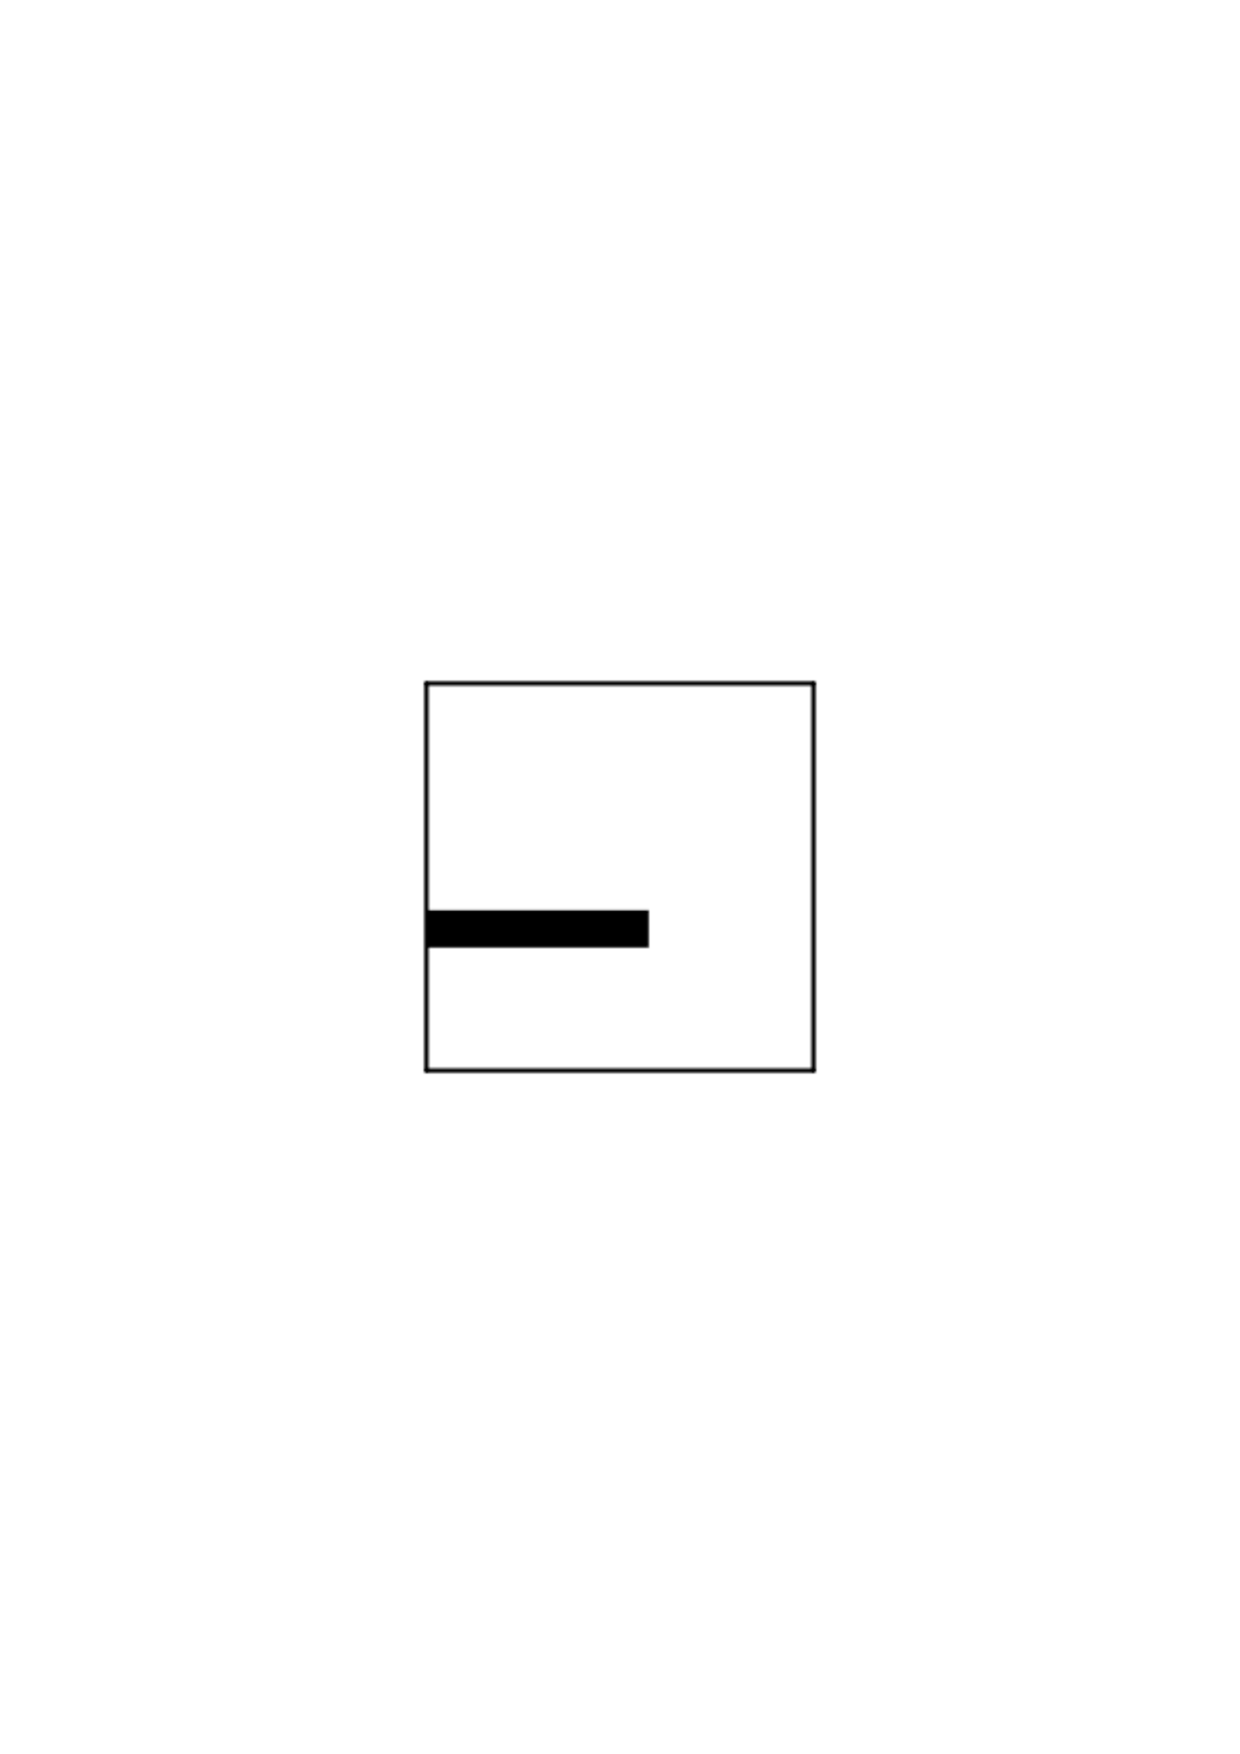
\includegraphics[width=0.25\columnwidth]{images/Fig1}
	\caption{Example visual stimulus}
	\label{figure:visualStimulus}
\end{figure}

The abstract coordinates are shown in Table~\ref{table:ply043CategoryParameters}. The auditory stimuli were 96 tones based on those used by \cite{Maddox2006}, that varied in duration and pitch. They were narrow-band noise, created by combining 50 independent phase sine waves. The frequencies of the stimuli were drawn from a normal distribution with a mean value of $F$ Hz and a standard deviation of $15.7$. $F$ were given by ${F = 1000*H + 150}$
where $H$ are the coordinates for height from the visual stimuli. The durations of the stimuli were given by the equation ${D = 2* (0.1 + 10^{L-1})}$, where $L$ are the arbitrary stimulus coordinates for length from the visual stimuli. 

\begin{table}[b!]
	\begin{center}
	\caption{Abstract category structures}
	\label{table:ply043CategoryParameters}
		\begin{tabular}[b]{c c c c c c}
			\hline\noalign{\smallskip}
			& \multicolumn{2}{c}{Height} & \multicolumn{2}{c}{Length} &\\
			& $\mu$ & $\sigma$ & $\mu$ & $\sigma$ & $cov_{xy}$ \\
			\noalign{\smallskip}\hline\noalign{\smallskip}
						\multicolumn{5}{l}{Conjunction} \\
			\noalign{\smallskip}
			A & 0.3 & 0.12 & 0.8 & 0.12 \\
			B & 0.3 & 0.12 & 0.4 & 0.12 \\ 
			B & 0.7 & 0.12 & 0.4 & 0.12 \\
			B & 0.7 & 0.12 & 0.8 & 0.12 \\
			\multicolumn{5}{l}{Information-integration} \\
			A & 3.1562 & 0.667 & 66.5 & 12.247 & 5\\
			B & 4.7546 & 0.667 & 37 & 12.247 & 5\\
			\noalign{\smallskip}\hline
		\end{tabular}
	\end{center}
\end{table}

The category structures were also counterbalanced. For the CJ structure, this resulted in four structures equivalent to rotating the category structure in Table~\ref{table:ply043CategoryParameters} by $\pi/2$ each time. 
There were 19 participants who assigned the top-left to Category A, 19 who assigned the top-right, 10 who assigned the bottom-left and 11 who assigned the bottom-right. 
For the II structure, there were two structures each a $\pi$ rotation of the other. 
There were 28 participants who learned a category structure with a positive correlation between dimensions and 30 that learned the rotation. 

\subsection{The questionnaire}

After they had completed the computer portion of the task, each participant answered the questions reproduced in Table~\ref{table:questionnaire}. 
Participants in the control condition completed the three relevant questions from the longer questionnaire.

\begin{table*}
	\centering
	\caption{Post-experiment verbal report questionnaire.}
	\label{table:questionnaire}
	\begin{tabular}{l p{0.7\textwidth} c}
		\toprule
		& Question & Type \\
		\midrule
		1 & Did you notice any relationship between the first part of the experiment (pictures) and the second part of the experiment (sounds)? & Yes/No\\
		2 & If your answer to Question 1 was YES, please describe the relationship below: & Open \\
		3 & For the first part of the experiment (pictures), are you able to describe how you decided whether a picture belonged in category A or category B? & Yes/No\\
		4 & If your answer to Question 3 was YES, please describe how you did it below: & Open \\
		5 & For the second part of the experiment (sounds),  are you able to describe how you decided whether a sound belonged in category A or category B?& Yes/No \\
		6 &  If your answer to Question 5 was YES, please describe how you did it below: & Open \\
		\bottomrule
	\end{tabular}
\end{table*}

We also asked two multiple choice questions about the visual and auditory tasks respectively. However, due to an error these were not interpretable and so have not been further considered.

Note that in previous experiments using these types of category structures, researchers have used a model-based decision-bound analysis informed by signal detection theory \citep{Ashby1988, Maddox1993}. However, recent work has shown that this analysis can be unreliable and consequently hard to interpret \citep{Donkin2015, Edmunds:2018kk}. Therefore, we have not included a description of this analysis in the main text, although it is available in the Appendix for those interested. 

\subsection{Materials}

The experiment was run on a PC connected to a 22-inch monitor with a 16:9 aspect ratio using E-Prime $2.0$. Responses were made  using a standard keyboard. The auditory stimuli were presented on Behringer  HPM1000 on-ear headphones. 

\subsection{Procedure}

Participants in the analogical transfer conditions completed both the training and test phases, whereas participants in the control condition only completed the test phase. The specific stimuli each participant was shown depended on the condition they were assigned. The training phase consisted of four blocks of 96 training trials. Participants were told they would be shown some `boxes' containing a single line and that their task was to identify the box as either Category A or Category B. Participants were also informed that the box stimuli would differ on two dimensions, height and length. Participants were told to indicate the category by pressing `Z' for Category A and `M' for Category B. Participants were told that they would have to guess which category each `box' belonged to at the start but that through corrective feedback they could achieve high accuracy.

On each trial, the participants were presented with a box stimulus for 1000 ms, which approximately matched the average duration of the auditory stimuli. This was replaced with the question ``Category A or Category B?'' This remained onscreen for 1000 ms. Once a response was detected, feedback was displayed for 1000 ms: either ``Correct'' in blue, or ``Incorrect'' in red as appropriate. If the participant failed to respond within 1000 ms, ``TIME OUT'' was displayed in red instead of feedback. The inter-trial interval was 500 ms.  There were no signals to indicate the end or beginning of an experimental block. 

The test phase consisted of a single block of 96 auditory stimuli. Participants were told that they would hear a series of sounds varying in duration and pitch. They were told that they would have to categorize the sounds by pressing ``Z'' for Category A or ``M'' for Category B. Participants did not receive feedback for this part of the experiment. 
As in \cite{Maddox2006}, the loudness of the stimuli were not controlled using a normalisation procedure.

On each trial, participants were presented with an auditory stimulus for the length of time specific to the stimulus. Then, the question ``Category A or Category B?'' was presented for 1000 ms, during which time the participant was allowed to respond. After receiving a response, a blank screen was presented for 1500 ms, before the start of the next trial.
However, if the participant failed to respond within 1000 ms, ``TIME OUT'' was displayed for 1000 ms followed by a blank screen for 500 ms. Before being debriefed, participants completed the short questionnaire about the experiment. 

\subsection{Analysis}

All data analyses were conducted in R \citep{Rcite}. Cohen's $d$ was calculated using the \texttt{effsize} R package \citep{effsize} and Bayes Factors using the \texttt{BayesFactor} package \citep{BayesFactor}. Bayes Factors ($BF_{10}$) exceeding three were considered evidence for the experimental hypothesis, while  $BF_{10} < \frac{1}{3}$  were considered evidence for the null; p-values are largely reported as a traditional courtesy, except where no Bayesian equivalent was known to us, in which case an alpha level of .05 was adopted. 
We also report generalised $\eta^2$. 
Trial by trial data, verbal reports and all analyses for this and three prior pilot experiments are available at \url{https://osf.io/mcd7v}.

\subsection{Results}

\subsubsection{Data rescoring}

A Shapiro-Wilks test showed that accuracy in the test phase in all four conditions violated assumptions of normality, $(p \leq .001)$. 
On visually inspecting the distributions of accuracy scores during the test phase, both conditions had distinctly bimodal distributions with peaks around $30\%$ and $70\%$. Matching peaks $20\%$ away from chance indicates that all participants were exhibiting systematic behavior related to the category structure, but were at chance on inferring which key went with which category label. 

There are two ways of solving this problem. One way is to use non-parametric tests. The other is to rescore the data so that it reflects difference from chance. This is where we think category learning differs from other research on analogical transfer. In `traditional' analogical transfer problems, such as the radiation problem, systematicity and accuracy are positively correlated. The more accurate you are, the better you have transferred the information from one task to another. In contrast, for a category learning task, systematicity forms a U-shaped curve on accuracy. Participants that score 100\% are also perfectly systematic, but so are those that score 0\%. Therefore, as we are interested in the `systematicity' of participants responses we chose the later approach. The rescored performance metrics `Systematic difference scores' are shown in Figure~\ref{figure:ply134learningCurveGraph} for the transfer conditions and Figure~\ref{fig:ply134transferGraph} for the test block. 

\subsubsection{Transfer}

\begin{figure}[t!]
	\centering
	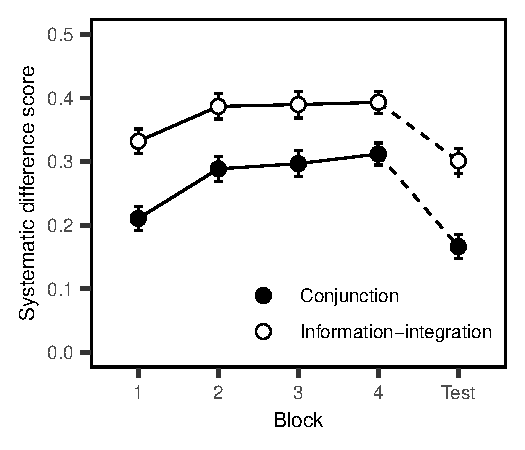
\includegraphics[width=0.4\textwidth]{images/ply134learningGraph.pdf}
	\caption{Learning curves of participants. Error bars are difference-adjusted between-subject 95\% confidence intervals \protect\citep{Baguley2012}.}
	\label{figure:ply134learningCurveGraph}	
\end{figure}


We conducted a 2 (task: CJ, II) x 2 (block: last training block, test) ANOVA on the data from the full condition. There was a main effect of block, $BF_{10}=1.4 \times 10^{8}, F(1, 57)=142.04, \eta^2=0.42, p<.001$: participants scored lower in the test block than at the end of training. There was also a main effect of category task, $BF_{10}=1.7 \times 10^6,  F(1,57) = 49.39, \eta^2=0.38, p<.001$ : participants scored higher on average in the II condition, $M_{II}=0.35, SD=0.08$, than in the CJ condition, $M_{CJ}=0.24, SD=0.10$. The evidence for an interaction was equivocal, $BF_{10}=1.61, F(1,57)=7.25, \eta^2 = 0.04, p=.009$.  The numerical trend was for performance to drop more in the rule-based (CJ) condition than in the II condition; this is opposite to the pattern reported in previous work.

\subsubsection{Comparison with controls}

Here, we examined whether training had any impact on final test performance. A 2 (Category structure: CJ, II) x 2 (Condition: Control, Experimental) ANOVA on test block accuracy found equivocal evidence for an interaction, $BF_{10}=0.43$, ${F(1,113)=1.03}$, ${\eta^2=0.01}$, ${p=.311}$, and evidence for the \emph{absence} of a main effect of condition, $BF_{10}=0.25$, ${F(1,113)=1.07}$, ${\eta^2=0.01}$, ${p=.302}$. There was a main effect of category structure, $BF_{10}=5.2 \times 10^{11}$, ${F(1, 113)=79.22}$, ${\eta^2=0.41}$, ${p<.001}$; participants scored higher on average on the II structure, $M_{II}=0.29$, $SD=0.07$, than on the CJ structure, $M_{CJ}=0.17$, $SD=0.08$. 

\begin{figure}[t!]
\centering
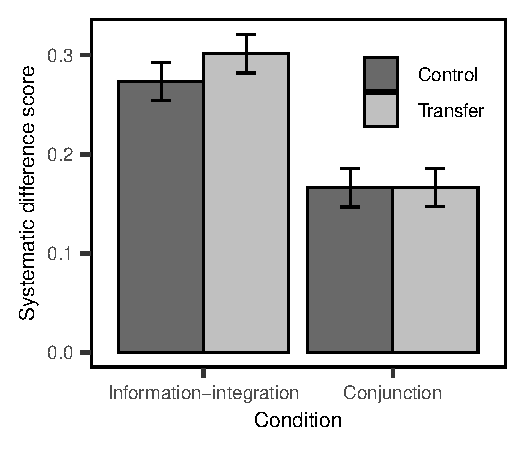
\includegraphics[width=0.45\textwidth]{images/PLY134transferGraph.pdf}	
\caption{Performance on the auditory test stimuli. Error bars are difference-adjusted between-subject 95\% confidence intervals \protect\citep{Baguley2012}.}
\label{fig:ply134transferGraph}
\end{figure}

\subsection{Verbal reports}

The open questions were coded by the first author (CERE) and a volunteer (MB). For the answer to Question~2, participants were identified by how they paired stimulus dimensions across the two phases of the experiment. For instance, ``short line matches short tone'' would have been coded as length-duration. The correct relationship was ``line length is tone duration and line position is tone pitch.''

For the answers to Questions~4 and 6, participants were identified as using one of the following strategies:

Participants were classified as using a {\it unidimensional} rule if they only mentioned a single stimulus dimension, such as ``if the line was short the stimulus was in Category A, if the line was long the stimulus was in Category B.''

Participants were classified as using a {\it conjunction} rule if they mentioned both stimulus dimensions and described categorizing stimuli on the basis of a logical ``AND'' rule such as ``short stimuli in the top half of the box were in Category A, otherwise they were in Category B.''

Participants were classified as using a {\it complex} rule if they mentioned both stimulus dimensions and described categorization stimuli on the basis of a series of complicated if statements, such as ``If the line is short it is in Category A, but if it is long it is in Category B. However, if it is mid-length then if it is high in the box it is Category B, and if it is low in the box it is in Category A.''

Participants were classified as {\it other} if they did not fall into one of the groups above. Inter-rater reliability was $82\%$. All discrepancies between raters were easily resolved following discussion.

Table~\ref{table:verbalReportRatePLY134} shows the proportion of participants that responded ``yes'' to the yes/no questions of Table~2, along with the corresponding statistical tests. 
There was evidence for the \emph{absence} of a difference between the CJ and II conditions in the proportions of participants that reported a strategy in the training phase. The same was true for the test phase. The evidence was equivocal for a difference between CJ and II in the proportion of participants who reported noticing a relationship between the two phases of the experiment. In the control conditions, numerically more people were able to report a strategy in the II task than in the CJ task, but the Bayesian evidence for that difference was equivocal

\begin{table}
	\centering
	\caption{Rows 1-3: Proportion of participants in the analogical transfer conditions responding 'yes' to verbal report questions 1, 3, and 5. Row 4: proportion of control participants responding 'yes' to their equivalent of question 5. The chi-squared test (and corresponding Bayes Factor) compare these proportions between categorization tasks.}
	\label{table:verbalReportRatePLY134}
	\begin{tabular}{l c c l c}
		\toprule
		& CJ & II & $\chi^2$ & $BF_{10}$ \\
                \midrule
		Q1. Relationship?  & 0.65 & 0.64 & 0.00 & 0.34\\          
		Q3. Strategy? (Training)  & 1.00 & 0.96 & 0.73 & 0.14\\
                Q5. Strategy? (Transfer) & 0.75 & 0.79 & 0.08 & 0.31\\                
		Q5. Strategy? (Controls) & 0.86 & 1.00 & 4.26 & 1.09 \\			
		\bottomrule
		\multicolumn{4}{p{0.33\textwidth}}{CJ = Conjunction, II = information-integration.}
	\end{tabular}
\end{table}

Next, we looked at the strategies participants reported (see Table~\ref{table:verbalsPLY134}).  No participants attempted to report anything that could even be loosely interpreted as implicit responding. Rather, for participants completing the full experiment, the majority of participants reported shifting from using two-dimensional rules during training to unidimensional rules at test. 
%There was no evidence to suggest that the rate of participants resorting in simpler strategies at test was different between category structure conditions, $BF_{10}=0.60$, $\chi^2=1.00$, $p=.318$.
In the CJ conditions, participants relied more on a unidimensional strategy in the control group than at test, $BF_{10}=4.12$, $\chi^2=4.95$, $p=.026$. In contrast, there was no evidence that this was the case in the II conditions, $BF_{10}=1.46$, $\chi^2=3.72$, $p=.054$. This interaction reached significance, $BF_{10}=7.15$, $\chi^2=12.65$, $p=.013$.
There was no evidence to suggest that participants relied less on the default unidimensional categorization strategy following CJ training than II training, $BF_{10}=1.31$, $\chi^2=2.58$, $p=.109$.

\begin{table}[t]
	\centering
		\caption{Proportion of participants reporting each strategy.}
	\label{table:verbalsPLY134}
	\begin{tabular}{l c c c c c}
		\toprule
		& & \multicolumn{4}{c}{Strategies} \\
		\cline{3-6} \\
		& Phase & UD & CJ & Complex & Other \\
		\midrule
		CJ & Training & 0.05 & 0.80 & 0.15 & - \\
		& Test & 0.47 & 0.40 & 0.13 & - \\
		& Control & 0.83 & - & 0.07 & 0.06 \\
		II & Training & 0.26 & 0.15 & 0.59 & -\\	
		& Test & 0.73 & 0.09 & 0.18 & - \\
		& Control & 0.93 & - & 0.07 & - \\
		\bottomrule
		\mc{6}{p{2.8in}}{Strategies: UD=Unidimensional, CJ=Conjunction, Complex=Complex multi-dimensional}
	\end{tabular}	
\end{table}

Finally, we looked at the proportion of participants in the full experiment conditions that were able to correctly specify the correct transfer mapping. In the rule-based condition, 38\% of participants correctly specified the transfer relationship, and 5\% of those in the II condition. The Bayesian evidence for this difference was equivocal, $BF_{10}=1.75$, $\chi^2=3.81$, $p=.051$. No participants were identified as using a different mapping (such as height of bar to length of tone). In the CJ condition, participants who reported the correct mapping performed worse, $M=0.14$, than those who reported an incorrect mapping, $M=0.18$, although the evidence for this difference equivocal, $BF_{10}=0.59$, $t(11)=-0.70$, $p=.501$.


\section{Discussion}

Analogical reasoning is crucial to transferring knowledge in many tasks and domains \citep{Barnett:2002io, Gentner:2018wo}. However, the role analogical reasoning plays in transferring category knowledge has only been partially explored. Some studies have explored analogical reasoning in near transfer, where the pre-transfer and post-transfer tasks are in the same context \citep{Casale:2012jf, Soto:2018up, Zakrzewski:2018gu}. They found that successful analogical transfer was contingent on the category structure: transfer was easier following UD training than II training. 

We extended the literature by investigating far transfer of category knowledge; in this case where category knowledge might have been transferred between two different modalities.
Participants were trained on a visual task and tested on an auditory task with the same underlying structure. 
There was evidence that, compared to the relevant control conditions, fewer participants used a unidimensional strategy in the CJ conditions than the II conditions. 
However, unlike the studies of near transfer, this did not result in improved accuracy: participants who received training on the visual task achieved the same levels of accuracy in the auditory task as those who did not receive training, irrespective of category structure.
 
The current findings contrast those in reasoning tasks, where analogical reasoning improves performance in the second task despite substantial changes in surface form \citep{Barnett:2002io, Gentner:2018wo}. 
This contrast may be due to task differences. 
In both kinds of task, participants might identify the optimum strategy, yet have problems implementing it. 
However, these problems of implementation seem likely to be more severe for a categorization task than a classic reasoning task. 
For example, knowing that ``small'' stimuli are in one category and ``large'' stimuli are in another can be hard to apply effectively if you do not know how small is ``small'' and how large ``large''. 
It it possible that these fine-grained adjustments require feedback. 

\subsection{Learning versus default strategy use}

In the control condition of the current experiment, classification of the auditory stimuli was performed in the absence of prior in-experiment training, and in the absence of feedback. 
We found, as others have previously \citep{Ashby:1999tka, Milton:2008hs, Wills2015}, that people do not guess in such situations, they instead apply a default, typically single-dimensional, strategy. 
It is reasonable to assume that they might at least start with a similar default strategy even when feedback is available. 
The issue this creates is that applying a single-dimension strategy to CJ and II category structures leads to substantially above-chance responding (optimally, 75\% correct for the current structures). 
This is important because learning is usually taken to mean some relatively permanent adaptation to the environment, rather than simply applying an existing strategy to a novel situation. 
Hence, one should not use above-chance responding in CJ and II tasks as evidence of category \emph{learning}, because an alternative explanation of above-chance responding is that participants applying an existing strategy. 
In the current work, the high performance of unidimensional strategies on a conjunction task mean that we may have inadvertently limited the possible performance benefit from training.
One possible solution to this issue would be to use category structures where unidimensional strategies score at chance levels \citep[\eg][]{Donkin2015}. 

\subsection{Relationship to the COVIS model}

According to the COVIS (COmpetition between Verbal and Implicit Systems) model \citep{Ashby1998}, the pattern of near transfer shown in \cite{Casale:2012jf}, \cite{Zakrzewski:2018gu} and \cite{Soto:2018up} occurs because different neural systems underlie performance in rule-based (UD and CJ) and II tasks. Participants can analogically transfer knowledge between different rule-based tasks because the Explicit System learns them using rules \citep{Ashby1998}. In contrast, participants fail to transfer knowledge of II tasks because they are learned by the implicit, Procedural System.

The results of the current study neither strongly support nor rule out the COVIS account. On one hand, consistent with COVIS, more people were able to report the correct relationship in the CJ condition than in the II condition (although the Bayesian evidence for this difference was inconclusive). On the other hand, COVIS hypothesizes that the II task is learned implicitly, yet most people reported using a rule-based strategy in this condition \citep[see also][]{Edmunds2015, Edmunds:2016tb, Edmunds:2018ek}.

Existing published accounts of COVIS are unclear about the possibility of cross-modal transfer of rule-based categories. On the one hand, cross-modal transfer is a form of analogical transfer, and analogical transfer of rule-based categories is expected and has been reported. On the other hand, the specific issue of cross-modal transfer in COVIS has not been covered in either published accounts or formal computational implementations. On the basis of the current results, we suggest that it may not be necessary to provide COVIS with a mechanism for cross-modal transfer.

\subsection{Conclusion}

In contrast to previous work on near analogical transfer \cite{Casale:2012jf, Soto:2018up, Zakrzewski:2018gu} in perceptual categorization, we found no beneficial effect of far, cross-modal, analogical transfer in either rule-based or information-integration category structures. 

\subsection{Author contributions}

\textbf{CERE} (lead author): Rationale, theory, design, programming, data collection, data analysis, writeup. \textbf{ABI}: Rationale, theory, design. Programming and analysis of pilot studies. \textbf{PMJ}: Design. \textbf{FM}: Rationale, theory, design. Consulted on analysis and write up as co-author. \textbf{AJW}: Rationale, theory, design, write up. Consulted on analysis. 


\bibliographystyle{apacite}
\bibliography{References}

\bigskip
\section*{Appendix}
\subsection*{Decision-bound strategy analyses}

Most studies in the COVIS canon include analysis of participants' strategies. This is required to patch a logical hole in the design of these experiments \citep{Edmunds:2018kk}. Recall that COVIS predicts the existence of two competing learning systems and that each system is hypothesised to optimally learn particular category structures. However, for any given COVIS experiment, there is no guarantee that participants are using the optimal system for the category structure they learn. Therefore, any dissociation in accuracy may reflect participants using the ``wrong'' system, rather than reflecting properties of the systems under study. To rule this possibility out, studies investigating the predictions of the COVIS model use a decision-bound model-based analysis to check that the strategies participants use are consistent with the category structure and the system they are supposed to be using.

This decision-bound strategy analysis is informed by a multi-dimensional version of signal detection theory: General Recognition Theory \citep{Ashby1988, Ashby1993}. Broadly, it involves fitting several different strategy models to the data from each participant and seeing which one fits the best. Following \cite{Casale:2012jf}, here we fitted three types of strategy: unidimensional, general linear classifier and random. Additionally, we also included a conjunction model as this would be the optimum strategy for the rule-based category structure used here. For ease of exposition, all strategies are framed in terms of the visual stimuli (an example is shown in Figure~\ref{figure:visualStimulus}, in the main text). 

\paragraph{Unidimensional} This strategy corresponds to a unidimensional rule such as ``Stimuli with short lines are in one category, those with long lines are in the other.'' Two parameters: position of the decision bound and noise. 

\paragraph{Conjunction} This strategy corresponds to a conjunction rule such as ``Stimuli with short lines high in the box are in Category A, otherwise they are in Category B.'' Three parameters: two defining the decision boundary plus noise. 

\paragraph{General linear classifier} Within the COVIS literature, this strategy is regarded as being learned implicitly. It corresponds to the strategy ``If the line is longer than it is high then it is in Category A, otherwise the stimulus is in Category B.'' Three parameters: two defining the decision boundary plus noise. 

\paragraph{Random} Two random models, one with one parameter (bias), one with no parameters. 

\vspace{12pt}

The best fit of these models was determined using the Bayesian Information Criterion. The best fitting models for each participant  are shown in Table~\ref{table:DBstrategyAnalysis}. Also reported are the Bayesian weights for the success of each model \citep{Wagenmakers:2004wn}. Code for these models fits are available at \url{https://osf.io/mcd7v}

\subsubsection*{Notes on interpretation}

The results of this strategy analysis are reported here for completeness and for comparison with other work investigating the COVIS model. However, as mentioned briefly in the main text, we have serious concerns about whether this form of strategy analysis accurately reflects the strategies that participants are using. Previous work, by ourselves and others, have shown that the output of this analysis critically depends on the category structure under consideration as well as the strategy models included, regardless of the strategies actually used by the participants \citep{Donkin2015, Edmunds:2018kk}. For instance, \cite{Edmunds:2018kk} found that approximately 50\% of simulated participants who learned an information-integration category structure using a rule-based strategy were misidentified by the analysis as using the optimum, diagonal strategy. Therefore, the strategies reported here should be interpreted very cautiously.


\begin{table*}
	\centering
	\caption{Decision-bound strategy analysis.}
	\label{table:DBstrategyAnalysis}
	\renewcommand{\arraystretch}{1.2}
	\begin{tabular}{C{1.5in}c C{0.8in}C{0.8in}C{0.8in}C{0.8in}}
		\toprule
		&Block&\multicolumn{4}{c}{Strategy {\it (wBIC)}}\\
		\cline{3-6}
		&& UD & CJ & GLC & RAND \\
		\midrule
		Conjunction & 4 & 0.10 {\it(0.70)}& 0.77 {\it(0.84)}& 0.13 {\it(0.60)}& - \\
		& Test & 0.57 {\it(0.72)}& 0.13 {\it(0.64)}& 0.07 {\it(0.47)}& 0.23 {\it(0.72)}\\
		& Control & 0.86 {\it(0.69)}& - & 0.03 {\it(0.54)}& 0.10 {\it(0.79)}\\
		Information-integration & 4 & 0.28 {\it(0.72)}& 0.10 {\it(0.68)}& 0.62 {\it(0.92)}& -\\
		& Test & 0.72 {\it(0.72)}& 0.07 {\it(0.49)}& 0.17 {\it(0.73)}& 0.03 {\it(0.76)}\\
		& Control & 0.97 {\it(0.72)}& - & - & 0.03 {\it(0.77)}\\
		\bottomrule
		\multicolumn{6}{p{5.2in}}{Strategies: UD=Unidimensional, CJ=Conjunction, GLC=Diagonal general linear classifier, RAND=Random.}
	\end{tabular}
\end{table*}


\end{document}

%%% Local Variables:
%%% mode: latex
%%% TeX-master: t
%%% End: